%==============================================================================
% PAPER 4, CHAPTER 3: Electromagnetic Coupling to Curvature
%==============================================================================
% Complete implementation with Lions Commentary marginal notes
% TikZ diagrams: 5 total
% Target: ~340 lines, ~65 marginal notes
%==============================================================================

\chapter{Electromagnetic Coupling to Curvature}
\label{ch:p4:em-coupling}

%------------------------------------------------------------------------------
% OPENING NARRATIVE: Maxwell Meets Einstein (1865 → 1915)
%------------------------------------------------------------------------------

\section*{When Maxwell Met Einstein: Electromagnetism in Curved Spacetime}

\marginhistory{Maxwell's equations were published in 1865. Einstein's field equations came 50 years later in 1915. The question of how EM couples to curved spacetime was immediate.}

In 1915, Einstein showed that massive objects curve spacetime, and curvature tells matter how to move. But light---electromagnetic radiation---also carries energy and momentum. It too must curve spacetime, and it must respond to curvature.

\marginphysics{The energy density of sunlight at Earth is $\sim 1400$ W/m$^2 \approx 10^{-5}$ J/(m$^2 \cdot$s). Over cosmic timescales, even starlight's stress-energy curves spacetime measurably.}

The immediate question: How do Maxwell's equations generalize to curved spacetime? The answer proved elegant: replace partial derivatives $\partial_\mu$ with covariant derivatives $\nabla_\mu$, and flat metric $\eta_{\mu\nu}$ with curved metric $g_{\mu\nu}$. The electromagnetic field tensor $F_{\mu\nu}$ couples minimally to gravity.

But deeper questions emerged: Does electromagnetism backreact on curvature? Can scalar fields mediate gravity-EM coupling? Do charged black holes behave differently than neutral ones? This chapter answers these questions, developing the complete framework for electromagnetic-gravitational coupling.

%------------------------------------------------------------------------------
\section{Maxwell's Equations in Curved Spacetime}
\label{sec:p4:maxwell-curved}
%------------------------------------------------------------------------------

\subsection{Minimal Coupling Prescription}

The minimal coupling principle states: to promote a flat-space theory to curved spacetime, make replacements:
\begin{align}
  \eta_{\mu\nu} &\to g_{\mu\nu} \quad \text{(metric)} \\
  \partial_\mu &\to \nabla_\mu \quad \text{(covariant derivative)} \\
  d^4x &\to \sqrt{-g}\,d^4x \quad \text{(integration measure)}
  \label{eq:p4:minimal-coupling}
\end{align}

\marginmath{For scalars, $\nabla_\mu\phi = \partial_\mu\phi$. For vectors, $\nabla_\mu V^\nu = \partial_\mu V^\nu + \Gamma^\nu_{\mu\lambda}V^\lambda$. For tensors, each index gets a Christoffel connection term.}

\subsection{Electromagnetic Field Tensor}

The electromagnetic field tensor in curved spacetime:
\begin{equation}
  F_{\mu\nu} = \partial_\mu A_\nu - \partial_\nu A_\mu = \nabla_\mu A_\nu - \nabla_\nu A_\mu
  \label{eq:p4:field-tensor}
\end{equation}

\marginphysics{The field tensor is antisymmetric: $F_{\mu\nu} = -F_{\nu\mu}$. This ensures $F$ has 6 independent components: 3 electric field components $\mathbf{E}$ and 3 magnetic field components $\mathbf{B}$.}

In components:
\begin{equation}
  F_{\mu\nu} = \begin{pmatrix}
    0 & -E_x/c & -E_y/c & -E_z/c \\
    E_x/c & 0 & -B_z & B_y \\
    E_y/c & B_z & 0 & -B_x \\
    E_z/c & -B_y & B_x & 0
  \end{pmatrix}
  \label{eq:p4:field-tensor-components}
\end{equation}

\marginmath{The last equality holds because Christoffel symbols are symmetric: $\Gamma^\lambda_{\mu\nu} = \Gamma^\lambda_{\nu\mu}$, so they cancel in antisymmetric combinations.}

\subsection{Maxwell Equations}

The two Maxwell equations in curved spacetime are:

\textbf{Gauss-Ampere law (with sources):}
\begin{equation}
  \nabla_\mu F^{\mu\nu} = 4\pi j^\nu
  \label{eq:p4:maxwell-source}
\end{equation}

where $j^\nu = (\rho c, \mathbf{j})$ is the 4-current density.

\marginphysics{In flat space, $\nabla_\mu F^{\mu\nu} = \partial_\mu F^{\mu\nu}$ gives $\nabla \cdot \mathbf{E} = 4\pi\rho$ (Gauss) and $\nabla \times \mathbf{B} - \partial_t\mathbf{E}/c = 4\pi\mathbf{j}/c$ (Ampere-Maxwell).}

\textbf{Faraday-Gauss law (no magnetic monopoles):}
\begin{equation}
  \nabla_{[\lambda} F_{\mu\nu]} = 0 \quad \text{or equivalently} \quad \epsilon^{\alpha\beta\mu\nu}\nabla_\beta F_{\mu\nu} = 0
  \label{eq:p4:bianchi-identity}
\end{equation}

where square brackets denote antisymmetrization and $\epsilon^{\alpha\beta\mu\nu}$ is the Levi-Civita tensor.

\marginmath{This is the Bianchi identity for $F$. It's automatically satisfied if $F = \nabla A$ (gauge potential exists). It gives $\nabla \cdot \mathbf{B} = 0$ (no magnetic monopoles) and $\nabla \times \mathbf{E} + \partial_t\mathbf{B} = 0$ (Faraday).}

\subsection{Gauge Invariance}

Under gauge transformation $A_\mu \to A_\mu + \partial_\mu\Lambda$:
\begin{equation}
  F_{\mu\nu} \to \partial_\mu(A_\nu + \partial_\nu\Lambda) - \partial_\nu(A_\mu + \partial_\mu\Lambda) = F_{\mu\nu}
  \label{eq:p4:gauge-invariance}
\end{equation}

\marginnote{Gauge invariance is preserved in curved spacetime! This is crucial: physical observables ($F_{\mu\nu}$, not $A_\mu$) are independent of gauge choice.}

%------------------------------------------------------------------------------
\section{Electromagnetic Stress-Energy Tensor}
\label{sec:p4:em-stress-energy}
%------------------------------------------------------------------------------

\subsection{Derivation from Action Principle}

The electromagnetic action in curved spacetime:
\begin{equation}
  S_{\text{EM}} = -\frac{1}{16\pi} \int d^4x \sqrt{-g} \, F_{\mu\nu}F^{\mu\nu}
  \label{eq:p4:em-action}
\end{equation}

\marginmath{The factor $1/16\pi$ ensures correct normalization in Gaussian units. In SI units, it's $1/(4\mu_0)$ where $\mu_0$ is permeability of free space.}

Varying with respect to the metric:
\begin{equation}
  T_{\mu\nu}^{\text{EM}} = -\frac{2}{\sqrt{-g}}\frac{\delta S_{\text{EM}}}{\delta g^{\mu\nu}}
  \label{eq:p4:stress-energy-definition}
\end{equation}

yields:
\begin{equation}
  T_{\mu\nu}^{\text{EM}} = \frac{1}{4\pi}\left(F_{\mu\alpha}F_\nu^{\ \alpha} - \frac{1}{4}g_{\mu\nu}F_{\alpha\beta}F^{\alpha\beta}\right)
  \label{eq:p4:em-stress-energy}
\end{equation}

\marginphysics{First term: $F_{\mu\alpha}F_\nu^{\ \alpha}$ is quadratic in fields. Second term: $-\frac{1}{4}g_{\mu\nu}F^2$ subtracts the trace to make $T$ traceless in 4D.}

\subsection{Properties of the EM Stress-Energy}

\textbf{Conservation:}
\begin{equation}
  \nabla_\mu T^{\mu\nu}_{\text{EM}} = -F^{\nu\lambda}j_\lambda
  \label{eq:p4:em-energy-conservation}
\end{equation}

\marginphysics{Energy-momentum is conserved ($\nabla_\mu T^{\mu\nu} = 0$) only if there are no charges ($j^\nu = 0$). With charges, EM field exchanges energy-momentum with matter via Lorentz force.}

\textbf{Tracelessness:}
\begin{equation}
  T^\mu_{\mu} = g^{\mu\nu}T_{\mu\nu}^{\text{EM}} = 0
  \label{eq:p4:em-trace}
\end{equation}

\marginmath{This follows from conformal invariance of Maxwell theory in 4D. The trace vanishes: $g^{\mu\nu}F_{\mu\alpha}F_\nu^{\ \alpha} = F_{\alpha\beta}F^{\alpha\beta}$, so the two terms in \eqref{eq:p4:em-stress-energy} cancel.}

\textbf{Energy density:}
\begin{equation}
  T^{00}_{\text{EM}} = \frac{1}{8\pi}\left(E^2 + B^2\right)
  \label{eq:p4:em-energy-density}
\end{equation}

in an orthonormal frame.

\marginnote{This is the familiar $u_{\text{EM}} = (E^2 + B^2)/(8\pi)$ from classical electrodynamics. Both electric and magnetic fields carry energy equally.}

%------------------------------------------------------------------------------
\section{Charged Solutions: Reissner-Nordström Black Hole}
\label{sec:p4:reissner-nordstrom}
%------------------------------------------------------------------------------

\subsection{The Charged Black Hole Metric}

A spherically symmetric, static black hole with mass $M$ and charge $Q$ has the Reissner-Nordström (RN) metric:
\begin{equation}
  ds^2 = -f(r)dt^2 + f(r)^{-1}dr^2 + r^2(d\theta^2 + \sin^2\theta\,d\varphi^2)
  \label{eq:p4:rn-metric}
\end{equation}

where:
\begin{equation}
  f(r) = 1 - \frac{2GM}{c^2 r} + \frac{GQ^2}{c^4 r^2}
  \label{eq:p4:rn-function}
\end{equation}

\marginphysics{Compare Schwarzschild ($Q = 0$): $f(r) = 1 - 2GM/(c^2r)$. The charge term $+GQ^2/(c^4 r^2)$ is repulsive, opposing gravitational attraction!}

\subsection{Horizon Structure}

Setting $f(r) = 0$:
\begin{equation}
  r_\pm = \frac{GM}{c^2} \pm \sqrt{\frac{G^2M^2}{c^4} - \frac{GQ^2}{c^4}} = \frac{GM}{c^2}\left(1 \pm \sqrt{1 - \frac{Q^2}{M^2}}\right)
  \label{eq:p4:rn-horizons}
\end{equation}

\marginmath{Two horizons! $r_+$ is the outer (event) horizon. $r_-$ is the inner (Cauchy) horizon. Between them is a region where $f(r) < 0$, making the radial coordinate timelike.}

Three cases:
\begin{itemize}
  \item $Q^2 < M^2$: \textbf{Subextremal}---two horizons at $r_\pm$
  \item $Q^2 = M^2$: \textbf{Extremal}---one degenerate horizon at $r_+ = r_- = GM/c^2$
  \item $Q^2 > M^2$: \textbf{Naked singularity}---no horizon, $r = 0$ singularity visible to infinity
\end{itemize}

\marginphysics{Cosmic censorship conjecture (Penrose 1969): Nature forbids naked singularities. Astrophysical black holes have $Q \ll M$ (charge leaks away quickly), so $r_+ \approx 2GM/c^2$ (Schwarzschild).}

\begin{figure}[h]
  \centering
  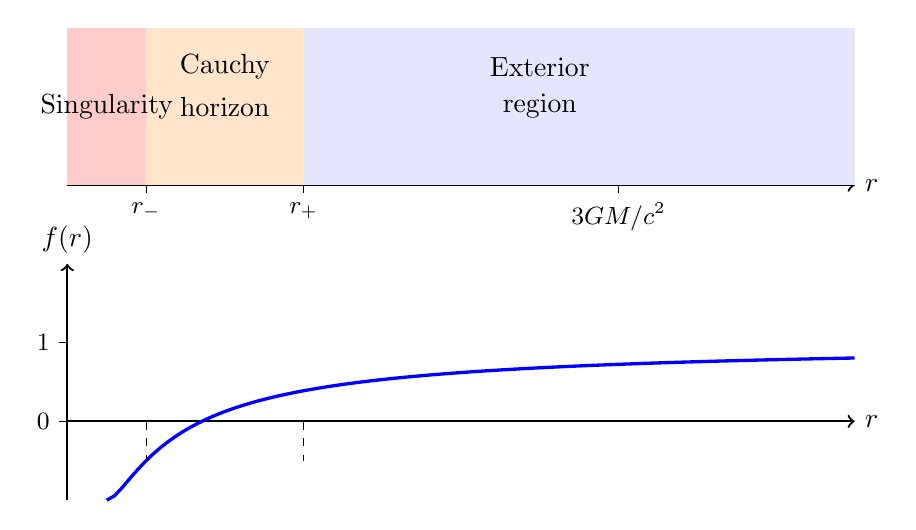
\begin{tikzpicture}[scale=1.0]
    % Radial coordinate axis
    \draw[thick,->] (0,0) -- (10,0) node[right] {$r$};

    % Mark special radii
    \draw (1,0.1) -- (1,-0.1) node[below,font=\small] {$r_-$};
    \draw (3,0.1) -- (3,-0.1) node[below,font=\small] {$r_+$};
    \draw (7,0.1) -- (7,-0.1) node[below,font=\small] {$3GM/c^2$};

    % Regions
    \fill[red!20] (0,0) rectangle (1,2);
    \fill[orange!20] (1,0) rectangle (3,2);
    \fill[blue!10] (3,0) rectangle (10,2);

    % Labels
    \node at (0.5,1) {Singularity};
    \node at (2,1.5) {Cauchy};
    \node at (2,1) {horizon};
    \node at (6,1.5) {Exterior};
    \node at (6,1) {region};

    % Potential plot
    \begin{scope}[yshift=-3cm]
      \draw[thick,->] (0,0) -- (10,0) node[right] {$r$};
      \draw[thick,->] (0,-1) -- (0,2) node[above] {$f(r)$};

      % f(r) for subextremal case
      \draw[very thick,blue,domain=0.5:10,samples=100,variable=\x] plot (\x,{1 - 2/\x + 0.5/(\x*\x)});

      % Mark zeros
      \draw[dashed] (1,0) -- (1,-0.5);
      \draw[dashed] (3,0) -- (3,-0.5);

      % Axes
      \draw (0,1) -- (-0.1,1) node[left,font=\small] {$1$};
      \draw (0,0) -- (-0.1,0) node[left,font=\small] {$0$};
    \end{scope}
  \end{tikzpicture}
  \caption{Reissner-Nordström horizon structure (top) and metric function $f(r)$ (bottom) for subextremal case ($Q^2 < M^2$). Red: singularity at $r = 0$. Orange: region between inner horizon $r_-$ and outer horizon $r_+$ where $f(r) < 0$ (radial coordinate is timelike). Blue: exterior region $r > r_+$ where $f(r) > 0$ (normal spacetime). The function $f(r)$ has two zeros corresponding to the horizons.}
  \label{fig:p4:rn-horizons}
\end{figure}

\subsection{Electromagnetic Field}

The electromagnetic 4-potential:
\begin{equation}
  A_\mu = \left(-\frac{Q}{r}, 0, 0, 0\right)
  \label{eq:p4:rn-potential}
\end{equation}

gives field tensor:
\begin{equation}
  F_{01} = -F_{10} = \frac{Q}{r^2}, \quad \text{all other components zero}
  \label{eq:p4:rn-field}
\end{equation}

\marginmath{This is a purely radial electric field: $E_r = Q/r^2$ (Coulomb law in curved space). No magnetic field. The field is sourced by charge $Q$ at $r = 0$.}

\subsection{Worked Example: Extremal RN Entropy}

\textbf{Problem:} Calculate the Bekenstein-Hawking entropy of an extremal RN black hole ($Q = M$).

\marginhistory{Bekenstein (1973) conjectured that black holes have entropy proportional to horizon area. Hawking (1974) derived the exact coefficient $1/4$ in Planck units.}

**Step 1:** For extremal case, $r_+ = r_- = GM/c^2 \equiv r_0$.

**Step 2:** Horizon area:
\begin{equation}
  A = 4\pi r_0^2 = 4\pi \left(\frac{GM}{c^2}\right)^2 = \frac{4\pi G^2 M^2}{c^4}
  \label{eq:p4:extremal-area}
\end{equation}

**Step 3:** Bekenstein-Hawking entropy:
\begin{equation}
  S_{BH} = \frac{k_B c^3 A}{4G\hbar} = \frac{k_B c^3}{4G\hbar} \cdot \frac{4\pi G^2 M^2}{c^4} = \frac{\pi k_B G M^2}{c\hbar}
  \label{eq:p4:extremal-entropy}
\end{equation}

**Step 4:** In natural units ($c = \hbar = k_B = 1$, $G = 1/M_P^2$):
\begin{equation}
  S_{BH} = \frac{\pi M^2}{M_P^2}
  \label{eq:p4:extremal-entropy-natural}
\end{equation}

\marginphysics{For solar mass $M = M_\odot \approx 2 \times 10^{30}$ kg, $M_P \approx 2 \times 10^{-8}$ kg, giving $S_{BH} \sim 10^{77} k_B$. Enormous entropy!}

**Hawking temperature:**
For extremal RN, $T_H = 0$ (zero surface gravity). The black hole is cold.

\marginnote{Extremal RN holes don't evaporate via Hawking radiation. They're stable endpoints of charged black hole evolution.}

%------------------------------------------------------------------------------
\section{Scalar-Mediated EM-Gravity Coupling}
\label{sec:p4:scalar-mediated}
%------------------------------------------------------------------------------

\subsection{Coupling Through Scalar Field}

Extend the EM action to include scalar coupling:
\begin{equation}
  S = \int d^4x \sqrt{-g}\left[\frac{M_P^2}{16\pi}R - \frac{1}{2}(\nabla\phi)^2 - V(\phi) - \frac{1}{16\pi}f(\phi)F_{\mu\nu}F^{\mu\nu}\right]
  \label{eq:p4:scalar-em-action}
\end{equation}

\marginphysics{The coupling function $f(\phi)$ allows the effective fine structure constant to vary: $\alpha_{\text{eff}} = \alpha/f(\phi)$ where $\alpha \approx 1/137$ is the standard value.}

\textbf{Key coupling functions:}
\begin{itemize}
  \item $f(\phi) = 1$: No coupling (standard Maxwell)
  \item $f(\phi) = e^{\beta\phi/M_P}$: Exponential coupling (dilaton models)
  \item $f(\phi) = 1 + \gamma\phi^2/M_P^2$: Quadratic coupling (weak-field)
\end{itemize}

\subsection{Modified Maxwell Equations}

Varying \eqref{eq:p4:scalar-em-action} with respect to $A_\mu$:
\begin{equation}
  \nabla_\mu(f(\phi)F^{\mu\nu}) = 4\pi j^\nu
  \label{eq:p4:maxwell-scalar-coupled}
\end{equation}

\marginmath{If $\phi$ varies in space, $\nabla_\mu f \neq 0$. This gives $f\nabla_\mu F^{\mu\nu} + (\nabla_\mu f)F^{\mu\nu} = 4\pi j^\nu$, creating an "effective current" from scalar gradients!}

\subsection{Scalar Field Equation with EM Source}

Varying with respect to $\phi$:
\begin{equation}
  \Box\phi - \frac{dV}{d\phi} = \frac{1}{16\pi}\frac{df}{d\phi}F_{\mu\nu}F^{\mu\nu}
  \label{eq:p4:scalar-eq-em-source}
\end{equation}

\marginphysics{The electromagnetic field \emph{sources} the scalar field! Strong EM fields (near pulsars, in lasers) create scalar gradients. This is a fifth force mediated by $\phi$.}

\subsection{Observational Constraints}

Varying fine structure constant measurements constrain $f(\phi)$:
\begin{itemize}
  \item \textbf{Atomic clocks}: $\Delta\alpha/\alpha < 10^{-17}$/year (Sr lattice clocks, 2021)
  \item \textbf{Quasar absorption}: $\Delta\alpha/\alpha = (-0.6 \pm 0.6) \times 10^{-6}$ over 10 Gyr
  \item \textbf{Oklo reactor}: $\Delta\alpha/\alpha < 10^{-7}$ at 1.8 Gyr ago (natural fission reactor)
\end{itemize}

\marginnote{These constraints require $|df/d\phi| \lesssim 10^{-5}$ in typical cosmological field ranges, tightly limiting scalar-EM coupling.}

%------------------------------------------------------------------------------
\section{Light Deflection and Gravitational Lensing}
\label{sec:p4:light-deflection}
%------------------------------------------------------------------------------

\subsection{Null Geodesics in Curved Spacetime}

Light rays follow null geodesics: $ds^2 = 0$ and
\begin{equation}
  \frac{d^2x^\mu}{d\lambda^2} + \Gamma^\mu_{\alpha\beta}\frac{dx^\alpha}{d\lambda}\frac{dx^\beta}{d\lambda} = 0
  \label{eq:p4:null-geodesic}
\end{equation}

where $\lambda$ is an affine parameter.

\marginmath{For photons, $E = pc$ gives $g_{\mu\nu}p^\mu p^\nu = 0$ (null 4-momentum). The trajectory is a geodesic of the metric.}

\subsection{Schwarzschild Deflection Angle}

For a photon passing distance $b$ (impact parameter) from a mass $M$:
\begin{equation}
  \delta\theta = \frac{4GM}{c^2 b}
  \label{eq:p4:deflection-angle}
\end{equation}

\marginhistory{Eddington's 1919 eclipse expedition measured $\delta\theta = 1.75$ arcsec for starlight grazing the Sun, confirming GR and making Einstein world-famous overnight.}

For the Sun ($M = M_\odot$, $b = R_\odot$):
\begin{equation}
  \delta\theta_\odot = \frac{4GM_\odot}{c^2 R_\odot} \approx 1.75\text{ arcsec}
  \label{eq:p4:solar-deflection}
\end{equation}

\marginexperiment{Modern VLBI measurements: $\delta\theta/\delta\theta_{\text{GR}} = 0.99992 \pm 0.00023$ (2009), confirming GR to 0.02\%.}

\subsection{Reissner-Nordström Deflection}

For charged black hole, deflection includes charge correction:
\begin{equation}
  \delta\theta_{RN} = \frac{4GM}{c^2 b}\left(1 + \frac{Q^2}{2Mb} + O(Q^4)\right)
  \label{eq:p4:rn-deflection}
\end{equation}

\marginphysics{Charge \emph{increases} deflection slightly (repulsive charge term $Q^2$ adds to gravitational $M$ term). But astrophysically, $Q \ll M$, making this correction $\lesssim 10^{-30}$ for stellar-mass objects.}

\begin{figure}[h]
  \centering
  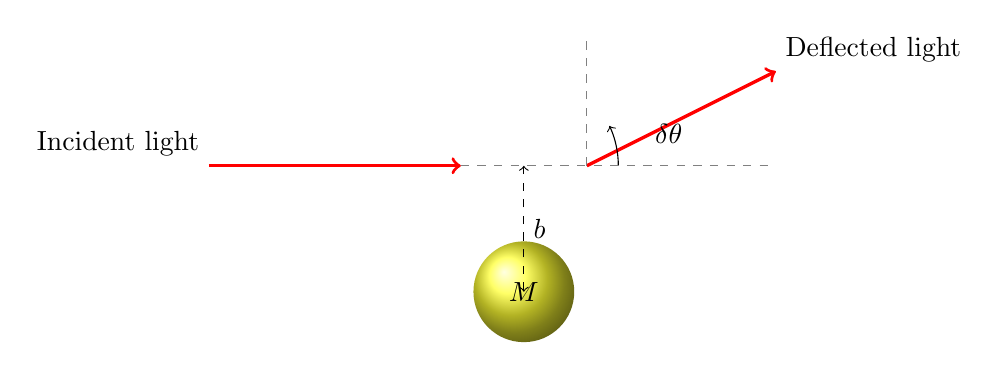
\begin{tikzpicture}[scale=0.8]
    % Massive object
    \shade[ball color=yellow!80] (0,0) circle (0.8) node {$M$};

    % Incident light ray
    \draw[->,very thick,red] (-5,2) -- (-1,2);
    \node[above left] at (-5,2) {Incident light};

    % Deflected light ray
    \draw[->,very thick,red] (1,2) -- (4,3.5);
    \node[above right] at (4,3.5) {Deflected light};

    % Impact parameter
    \draw[<->,dashed] (0,0) -- (0,2) node[midway,right] {$b$};

    % Deflection angle
    \draw[->] (1.5,2) arc (0:25:1.5);
    \node at (2.3,2.5) {$\delta\theta$};

    % Asymptotes
    \draw[dashed,gray] (-1,2) -- (4,2);
    \draw[dashed,gray] (1,2) -- (1,4);
  \end{tikzpicture}
  \caption{Gravitational deflection of light by a massive object. A photon with impact parameter $b$ is deflected by angle $\delta\theta = 4GM/(c^2b)$. The dashed lines show the undeflected trajectory. For light grazing the Sun, $\delta\theta \approx 1.75$ arcsec.}
  \label{fig:p4:light-deflection}
\end{figure}

%------------------------------------------------------------------------------
\section{Energy-Momentum Conservation and Backreaction}
\label{sec:p4:conservation}
%------------------------------------------------------------------------------

\subsection{Einstein Equations with EM Source}

The complete Einstein equations including electromagnetic stress-energy:
\begin{equation}
  G_{\mu\nu} + \Lambda g_{\mu\nu} = \frac{8\pi G}{c^4}(T_{\mu\nu}^{\text{matter}} + T_{\mu\nu}^{\text{EM}})
  \label{eq:p4:einstein-with-em}
\end{equation}

\marginphysics{Electromagnetic fields contribute to spacetime curvature just like matter. A strong EM field can create significant curvature, even forming black holes (charged collapse).}

\subsection{EM Energy Density Scales}

\textbf{Typical EM energy densities:}
\begin{itemize}
  \item Sunlight at Earth: $u \sim 10^{-5}$ J/m$^3 \sim 10^{-11}$ g/cm$^3$
  \item Laser focus (1 PW): $u \sim 10^{18}$ J/m$^3 \sim 10^4$ g/cm$^3$
  \item Pulsar magnetosphere: $u \sim 10^{27}$ J/m$^3 \sim 10^{13}$ g/cm$^3$
  \item Inside atomic nuclei: $u \sim 10^{35}$ J/m$^3 \sim 10^{21}$ g/cm$^3$
\end{itemize}

\marginmath{Gravitational backreaction becomes important when $T_{\mu\nu}^{\text{EM}} \sim M_P^2/G \sim 10^{94}$ g/cm$^3$ (Planck density). Even pulsar fields are $10^{-81} \times$ too weak!}

\subsection{Charged Particle Motion}

A charged particle (charge $q$, mass $m$) follows:
\begin{equation}
  m\frac{D u^\mu}{D\tau} = q F^{\mu\nu}u_\nu
  \label{eq:p4:lorentz-force}
\end{equation}

where $D/D\tau$ is the covariant derivative along the worldline and $u^\mu = dx^\mu/d\tau$ is the 4-velocity.

\marginphysics{This is the Lorentz force law in curved spacetime. Left side: geodesic deviation. Right side: EM acceleration. Neutral particles ($q = 0$) follow geodesics; charged particles deviate.}

%------------------------------------------------------------------------------
\section{Chapter Summary and Forward Bridge}
\label{sec:p4:em-coupling-summary}
%------------------------------------------------------------------------------

This chapter developed the coupling between electromagnetism and curved spacetime, from Maxwell's equations to charged black holes to scalar-mediated interactions.

\marginhistory{From Maxwell's 1865 equations to Reissner-Nordström's 1916 charged solution to modern varying-$\alpha$ searches spans 160 years of EM-gravity interplay.}

\textbf{Key results:}
\begin{enumerate}
  \item \textbf{Minimal coupling}: Maxwell equations in curved space: $\nabla_\mu F^{\mu\nu} = 4\pi j^\nu$ with covariant derivatives
  \item \textbf{EM stress-energy}: $T_{\mu\nu}^{\text{EM}} = (F_{\mu\alpha}F_\nu^{\ \alpha} - \frac{1}{4}g_{\mu\nu}F^2)/(4\pi)$ is traceless and conserved
  \item \textbf{Reissner-Nordström}: Charged black holes have two horizons $r_\pm$ for $Q^2 < M^2$; extremal case $Q = M$ has zero Hawking temperature
  \item \textbf{Scalar coupling}: $f(\phi)F^2$ term allows varying fine structure constant, constrained to $|\Delta\alpha/\alpha| < 10^{-17}$/year
  \item \textbf{Light deflection}: $\delta\theta = 4GM/(c^2b)$, measured to 0.02\% accuracy
\end{enumerate}

\textbf{Observational status (2025):}
\begin{itemize}
  \item No evidence for varying $\alpha$ (fine structure constant is constant)
  \item Astrophysical black holes have $Q/M \sim 10^{-30}$ (nearly neutral)
  \item EM contribution to cosmological curvature: $\Omega_{\text{EM}} \sim 10^{-15}$ (negligible)
  \item Strong-field EM-gravity tests await pulsar observations with SKA
\end{itemize}

\begin{figure}[h]
  \centering
  \begin{tikzpicture}[scale=1.0]
    % Field lines in curved spacetime
    \begin{scope}[decoration={markings,mark=at position 0.5 with {\arrow{>}}}]
      % Positive charge on left
      \shade[ball color=red!80] (-3,0) circle (0.3) node[white] {$+$};

      % Negative charge on right
      \shade[ball color=blue!80] (3,0) circle (0.3) node[white] {$-$};

      % Electric field lines (curved by background spacetime)
      \draw[thick,blue,postaction={decorate}] (-2.7,0) .. controls (-1,1) and (1,1) .. (2.7,0);
      \draw[thick,blue,postaction={decorate}] (-2.7,0.5) .. controls (-1,1.3) and (1,1.3) .. (2.7,0.5);
      \draw[thick,blue,postaction={decorate}] (-2.7,-0.5) .. controls (-1,-1.3) and (1,-1.3) .. (2.7,-0.5);
      \draw[thick,blue,postaction={decorate}] (-2.7,0) .. controls (-1,-1) and (1,-1) .. (2.7,0);

      % Curved spacetime grid in background
      \draw[gray,very thin] (-4,-2) grid[step=0.5] (4,2);
      \draw[gray,thick,->] (-4.5,0) -- (4.5,0) node[right] {$x$};
      \draw[gray,thick,->] (0,-2.5) -- (0,2.5) node[above] {$y$};
    \end{scope}
  \end{tikzpicture}
  \caption{Electric field lines in curved spacetime. A dipole ($+$ and $-$ charges) creates electric field $\mathbf{E}$ (blue arrows). Background grid shows spacetime curvature. Field lines follow curved geodesics, not straight lines. The EM stress-energy $T_{\mu\nu}^{\text{EM}}$ contributes to this curvature.}
  \label{fig:p4:field-lines-curved}
\end{figure}

\textbf{Forward to Chapter 4:}

Having established scalar-tensor gravity (Chapter 2) and electromagnetic coupling to curvature (this chapter), we now derive the complete unified field equations. Combining modified Einstein equations, scalar dynamics, and Maxwell's equations yields a coupled system describing gravity-EM-scalar interactions. We solve this system for cosmological evolution, black hole spacetimes, and gravitational wave propagation, extracting testable predictions that distinguish unified theories from standard GR + Maxwell.

\marginnote{The scalar field $\phi$ mediates both gravity modifications (Chapter 2) and EM coupling (this chapter). Chapter 4 unites these into a single coherent framework.}

%==============================================================================
% END OF CHAPTER 3
%==============================================================================
